\documentclass[11pt]{article}
\usepackage[a4paper, margin=1in]{geometry}
\usepackage{amsmath, amssymb}
\usepackage{xcolor}
\usepackage{tcolorbox}
\usepackage{tikz}
\usetikzlibrary{angles, quotes}

\definecolor{main}{RGB}{20, 70, 160}
\definecolor{accent}{RGB}{200, 60, 60}
\definecolor{soft}{RGB}{245, 247, 255}

\title{\textbf{\textcolor{main}{Law of Cosines Handout}}\\
\large \textcolor{accent}{Simple Rigour}}
\author{Lostless1907}
\date{20 April 2026}

\begin{document}

\maketitle
\vspace{-1em}

\begin{tcolorbox}[colback=soft, colframe=main]
\textbf{Big Idea.} We are not memorizing a formula.

We will \textit{build} it using:
\begin{itemize}
\item points on a graph
\item distance formula
\item basic trig ($\cos, \sin$)
\end{itemize}
\end{tcolorbox}

\section*{\textcolor{main}{Place the Triangle Smartly}}

We take a triangle and place it on a coordinate plane.

\begin{center}
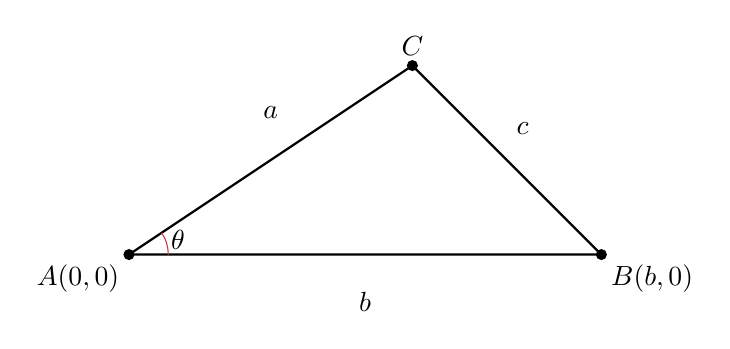
\begin{tikzpicture}[scale=2]

\coordinate (A) at (0,0);
\coordinate (B) at (3,0);
\coordinate (C) at (1.8,1.2);

\draw[thick] (A) -- (B) -- (C) -- cycle;

\fill (A) circle (1pt) node[below left] {$A(0,0)$};
\fill (B) circle (1pt) node[below right] {$B(b,0)$};
\fill (C) circle (1pt) node[above] {$C$};

\draw pic[draw=accent, "$\theta$", angle eccentricity=1.3] {angle = B--A--C};

\node at (1.5, -0.3) {$b$};
\node at (0.9, 0.9) {$a$};
\node at (2.5, 0.8) {$c$};

\end{tikzpicture}
\end{center}

\textbf{What we fixed:}
\begin{itemize}
\item $A = (0,0)$
\item $B = (b,0)$
\item $AC = a$, $AB = b$, $BC = c$
\end{itemize}

\textbf{Why?} One side is flat on the $x$-axis → less confusion.

\section*{\textcolor{main}{Where is Point $C$?}}

We know:
\begin{itemize}
\item length $AC = a$
\item angle at $A$ is $\theta$
\end{itemize}

So point $C$ must be:

\[
C = (a\cos\theta,\; a\sin\theta)
\]

\begin{tcolorbox}[colback=soft, colframe=accent]
\textbf{Simple meaning:}

\begin{itemize}
\item $a\cos\theta$ = how far right we go
\item $a\sin\theta$ = how far up we go
\end{itemize}

This is just ``walk $a$ units at angle $\theta$''.
\end{tcolorbox}
\section*{\textcolor{main}{Where does the Distance Formula Come From?}}

Take two points:
\[
P(x_1, y_1), \quad Q(x_2, y_2)
\]

Draw a right triangle:

\begin{center}
\begin{tikzpicture}[scale=2]

\coordinate (P) at (0,0);
\coordinate (Q) at (2,1.5);
\coordinate (R) at (2,0);

\draw[thick] (P) -- (Q);
\draw[dashed] (P) -- (R) -- (Q);

\fill (P) circle (1pt) node[below left] {$P(x_1,y_1)$};
\fill (Q) circle (1pt) node[above right] {$Q(x_2,y_2)$};
\fill (R) circle (1pt) node[below right] {$R$};

\node at (1,-0.2) {$x_2 - x_1$};
\node at (2.2,0.75) {$y_2 - y_1$};

\end{tikzpicture}
\end{center}

\textbf{What is happening:}

\begin{itemize}
\item Horizontal change = $x_2 - x_1$
\item Vertical change = $y_2 - y_1$
\end{itemize}

So we made a right triangle where:
\begin{itemize}
\item base = $x_2 - x_1$
\item height = $y_2 - y_1$
\item hypotenuse = distance between $P$ and $Q$
\end{itemize}

By Pythagoras:

\[
\text{distance}^2 = (x_2 - x_1)^2 + (y_2 - y_1)^2
\]

\begin{tcolorbox}[colback=soft, colframe=accent]
\[
\boxed{d^2 = (x_2 - x_1)^2 + (y_2 - y_1)^2}
\]
\end{tcolorbox}

\section*{\textcolor{main}{Turn Geometry into Distance}}

We now find side $c = BC$ using distance formula.

\[
c^2 = (x_2 - x_1)^2 + (y_2 - y_1)^2
\]

Between $B(b,0)$ and $C(a\cos\theta, a\sin\theta)$:

\[
c^2 = (a\cos\theta - b)^2 + (a\sin\theta)^2
\]

\section*{\textcolor{main}{Expand Slowly, painful but work out the algebra YOURSELF}}

\[
c^2 = a^2\cos^2\theta - 2ab\cos\theta + b^2 + a^2\sin^2\theta
\]

Group:

\[
c^2 = a^2(\cos^2\theta + \sin^2\theta) + b^2 - 2ab\cos\theta
\]

Now the only identity we use:

\[
\cos^2\theta + \sin^2\theta = 1
\]

So,

\[
c^2 = a^2 + b^2 - 2ab\cos\theta
\]

\begin{tcolorbox}[colback=soft, colframe=main]
\[
\boxed{c^2 = a^2 + b^2 - 2ab\cos\theta}
\]
\end{tcolorbox}

\section*{\textcolor{main}{Visual Meaning}}

\begin{center}
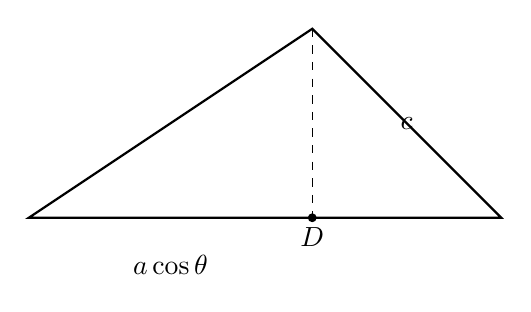
\begin{tikzpicture}[scale=2]

\coordinate (A) at (0,0);
\coordinate (B) at (3,0);
\coordinate (C) at (1.8,1.2);
\coordinate (D) at (1.8,0);

\draw[thick] (A) -- (B) -- (C) -- cycle;
\draw[dashed] (C) -- (D);

\fill (D) circle (0.8pt) node[below] {$D$};

\node at (0.9, -0.3) {$a\cos\theta$};
\node at (2.4, 0.6) {$c$};

\end{tikzpicture}
\end{center}

\textbf{Interpretation:}

\begin{itemize}
\item $a\cos\theta$ = projection of side $a$ onto base
\item The term $-2ab\cos\theta$ adjusts for how much the triangle ``leans''
\end{itemize}

\section*{\textcolor{main}{Physics}}

Think of sides as vectors.

\[
c^2 = |\vec{a} - \vec{b}|^2
\]

Expand:

\[
= a^2 + b^2 - 2ab\cos\theta
\]

\begin{tcolorbox}[colback=soft, colframe=accent]
\textbf{Meaning:}

Cosine measures how much one side goes in the direction of the other.

More alignment → smaller $c$.

More opposite → larger $c$.
\end{tcolorbox}

\section*{\textcolor{main}{Final Thoughts}}

\begin{center}
\textcolor{accent}{This is formula is on the edge of Physics and Math}

\vspace{0.3em}

\textcolor{main}{Peak Shi}
\end{center}

\end{document}
